\documentclass{article}
\author{Mgr. Ľuboš Valo}
\usepackage{ragged2e}
\usepackage{showframe}
\usepackage{amssymb}
\usepackage[none]{hyphenat}
\usepackage{microtype}
\usepackage{breqn}
\usepackage{mathtools}

\usepackage{graphicx}
\graphicspath{
    {../../../media/images/}
}

\overfullrule=5pt

\title{Číselné sústavy}
\begin{document}

\maketitle

\section{Číselné sústavy}

Číslica je symbol, ktorým zapisujeme hodnotu v danej sústave.

Číselné sústavy vznikli z potreby človeka počítať, porovnávať množstvo a zaznamenávať údaje. Prvé spôsoby vyjadrovania počtu boli veľmi jednoduché. Pravekí ľudia používali napríklad zárezové značky do kostí, kameňov alebo dreva, pričom každý zárez predstavoval jednu vec. Tento spôsob bol vhodný len na malé počty, pretože pri väčších množstvách sa stal neprehľadným.

Postupne vznikali dokonalejšie číselné sústavy, ktoré využívali skupiny znakov na označenie väčších hodnôt. Jednou z najstarších známych bola sumerská šesťdesiatková sústava, ktorá používala základ 60. Jej pozostatky sa zachovali napríklad v dnešnom meraní času (60 sekúnd v minúte, 60 minút v hodine) alebo uhlov (360 stupňov v kruhu).

Starovekí Egypťania používali desiatkovú nepozičnú sústavu, v ktorej mali osobitné symboly pre jednotky, desiatky, stovky a ďalšie hodnoty. Hodnota znaku nezávisela od jeho polohy v zápise.

Významným krokom vo vývoji bola rímska číselná sústava, ktorá používala znaky ako I, V, X, L, C, D a M. Táto sústava sa používa dodnes napríklad pri označovaní kapitol, hodín alebo významných udalostí, no pre zložitejšie výpočty nie je praktická.

Neskôr vznikli pozičné číselné sústavy, pri ktorých hodnota číslice závisí od jej polohy v čísle. Najdôležitejšou z nich sa stala desiatková sústava, ktorú používame dnes. Jej základ tvorí desať číslic (0–9) a každá pozícia predstavuje určitú mocninu čísla 10.

S rozvojom matematiky a techniky sa začali používať aj ďalšie pozičné sústavy, napríklad dvojková sústava, ktorá sa stala základom fungovania počítačov, pretože pracuje iba s dvoma hodnotami – 0 a 1. Okrem nej sa v informatike využívajú aj osmičková a šestnástková sústava, ktoré uľahčujú zápis dlhých binárnych čísel.

Vývoj číselných sústav teda prešiel od jednoduchých značiek na počítanie až k moderným systémom, ktoré umožňujú fungovanie dnešných počítačov a digitálnych technológií.

\subsection{Nepozičné číselné sústavy}

\subsection{Unárna číselná sústava}

Unárna číselná sústava (nazývaná aj jednotková číselná sústava) je najjednoduchšia a pravdepodobne najstaršia forma zapisovania čísel. Je to nepozičná číselná sústava, ktorá na vyjadrenie počtu používa iba jeden symbol. Hodnota čísla sa rovná počtu použitých symbolov.

Napríklad pri použití symbolu $\vert$ sa čísla zapisujú takto:
\begin{align*}
  1 &= \vert \\
  2 &= \vert \vert \\
  3 &= \vert \vert \vert \\ 
  4 &= \vert \vert \vert \vert \\
  5 &= \vert \vert \vert \vert \vert \\
  & \hspace{5pt} \vdots \\
  10 &= \vert \vert \vert \vert \vert \vert \vert \vert \vert \vert \vert \\
\end{align*}


Unárna sústava sa používala už v praveku, napríklad vo forme zárezov do kostí, dreva alebo kameňov pri evidovaní počtu zvierat, dní alebo predmetov. S podobným spôsobom zápisu sa stretávame aj dnes, napríklad pri ručnom počítaní hlasov alebo bodov pomocou čiarok.

Hlavnou výhodou unárnej sústavy je jej jednoduchosť a názornosť. Nevýhodou je však neefektívnosť pri zapisovaní väčších čísel, pretože počet symbolov rýchlo narastá, a tiež problematický zápis čísel iných než celých. Preto bola nahradená číselnými sústavami, ako sú desiatková alebo dvojková sústava.


\subsection{Aditívna číselná sústava}

Aditívna číselná sústava je typ nepozičnej číselnej sústavy, v ktorej sa hodnota čísla určuje sčítaním hodnôt jednotlivých symbolov bez ohľadu na ich pozíciu v zápise. Každý symbol má pevnú hodnotu a výsledné číslo vznikne súčtom všetkých použitých symbolov. Dodnes sa používajú napríklad pri peniazoch a rímskych číslach.

Príkladom aditívnej sústavy je staroegyptská číselná sústava. Egypťania používali rôzne hieroglyfy pre jednotky, desiatky, stovky, tisíce a ďalšie hodnoty. Ak chceli zapísať číslo \(243\), použili dva symboly pre stovky, štyri symboly pre desiatky a tri symboly pre jednotky. Hodnota čísla sa získala ich sčítaním:

\[
243 = 200 + 40 + 3.
\]

Egyptský hieroglyfický číselný systém obsahoval čísla \(1\), \(10\), \(100\), \(1\ 000\), \(10\ 000\), atď.

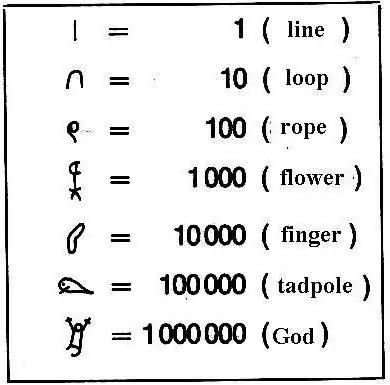
\includegraphics[width=100pt]{Staroegyptská číselná sústava.png}

Egyptský číselný systém

Podobný princíp využíva aj rímska číselná sústava. Rímska číselná sústava je historická nepozičná číselná sústava, ktorú používali obyvatelia starovekého Ríma. Na zapisovanie čísel využíva písmená latinskej abecedy, pričom každé písmeno má určenú číselnú hodnotu. Základné rímske číslice sú:

\begin{table}[h]
\centering
\begin{tabular}{c|ccccccc}
\hline
Symbol & I & V & X & L & C & D & M \\
\hline
Hodnota & 1 & 5 & 10 & 50 & 100 & 500 & 1000 \\
\hline
\end{tabular}
\caption{Rímske číslice a ich hodnoty.}
\end{table}
Mnemotechnická pomôcka: LaCo DoMa


Rímska číselná sústava je o niečo zložitejšia. Nie je úplne čisto nepozičná, ak ju chápeme podľa všetkých historických pravidiel. Tradične sa označuje ako nepozičná sústava, pretože väčšina znakov má stálu hodnotu bez ohľadu na miesto. Číslica X má vždy hodnotu 10. Avšak existujú zápisy, kde poradie číslic určuje ich význam.

Poznáme dva typy zápisu rímskych čísel: sčítací (tzv. aditívny) a odčítací (tzv. subtraktívny).

V sčítacom tvare má každá číslica stálu hodnotu, bez ohľadu na jej pozíciu v čísle. Na zápis čísla \(3738\) v čo najkratšom tvare sa použijú tri symboly M, jeden symbol D, dva symboly C, tri symboly X, jeden symbol V a tri symboly I. Vznikne tak rímske číslo MMMDCCXXXVIII. Sčítaním jednotlivých číslic by sme dostali:

\begin{align*}
  MMMDCCXXXVIII &= MMM + D + CC + XXX + V + III, \\
  3738 &= 3000 + 500 + 200 + 30 + 5 + 3.
\end{align*}

\[
3738 = 3000 + 500 + 200 + 30 + 5 + 3
\]

Toto číslo by sa dalo zapísať aj ako MMDMCXIXVIXIC. Z dôvodu prehľadnosti sa najväčšie číslice vždy píšu pred menšími.

V odčítacom tvare záleži na tom, či je menšia číslica pred väčšou. Ak sa menšia rímska číslica nachádza pred väčšou, jej hodnota sa od väčšej odčíta namiesto toho, aby sa sčítala. Napríklad číslo \(9\) by sa v odčítacom tvare zapísalo ako IX.

Rímska sústava používaná dnes je aditívno-subtraktívna. To znamená, že číslice sa väčšinou sčítavajú, ale v niektorých prípadoch sa menšia číslica pred väčšou odčítava. Platia nasledovné pravidlá:

\begin{itemize}
  \item Ak je menšia alebo rovnaká číslica za väčšou, hodnoty sa sčítajú. Číslo VIII znamená \(5 + 1 + 1 + 1 = 8\).
  \item Ak je menšia číslica pred väčšou, od väčšej sa odčíta. Číslo XXIX znamená \(10 + 10 + 10 - 1 = 29\). Správne kombinácie:
\begin{center}
\begin{tabular}{|c|c|c|c|c|c|c|}
IV & IX & XL & XC & CD & CM \\
4 & 9 & 40 & 90 & 400 & 900 \\
\end{tabular}
\end{center}
Iné odčítacie kombinácie sa nepoužívajú.
  \item Číslice I, X, C, M sa môžu opakovať najviac trikrát za sebou. Číslice V, L, D sa neopakujú.
  \item Číslice sa zapisujú od najväčšej hodnoty k najmenšej, s výnimkou povolených odčítacích dvojíc.
  \item Rímska sústava nemá vlastný symbol pre nulu. Nula sa v klasickom rímskom zápise nepoužívala.
\end{itemize}

Rímske číslice sa používajú dodnes najmä na označovanie, nie na bežné počítanie. V modernej matematike ich nahradila desiatková pozičná sústava, ale zostali zachované v niektorých oblastiach tradície a označovania. Najčastejšie sa používajú na ciferníky hodín, označenie panovníkov a pápežov, číslovanie kapitol a častí kníh, filmy, seriály a pokračovania diel, športové a kultúrne podujatia, roky na budovách a pamätníkoch a chemické, vedecké a technické označenia.

Nepozičné číselné sústavy majú oproti pozičným číselnym sústavam nevýhodu v tom, že je zložité zapisovanie veľkých čísel a ťažšie sa s nimi vykonávajú matematické výpočty.

\subsection{Pozičné číselné sústavy}

Pozičná číselná sústava je taká číselná sústava, v ktorej hodnota číslice závisí od jej polohy (pozície) v čísle. Každá pozícia má určitú hodnotu danú základom sústavy. Preto môže mať tá istá číslica rôznu hodnotu podľa toho, kde sa nachádza.

Základ číselnej sústavy. Každá pozičná sústava má svoj základ. Základ určuje, koľko rôznych číslic sústava používa. Každá číslica sama o sebe vyjadruje nejakú určitú hodnotu. Napríklad čislica \(6\) v desiatkovej sústave vyjadruje početnosť šesť. Jej pozícia v čísle mení jej hodnotu. V čísle \(60\) je šestka na pozícií desiatok, vyjadruje teda desaťnásobne väčšiu hodnotu, ako je hodnota \(6\).

Pozícia (miesto) číslice. Pozícia určuje, akú hodnotu má číslica v čísle.

Rád číslice. Rád určuje mocninu základu, ktorá patrí danej pozícii.

Hodnota číslice v pozícii. Celková hodnota číslice vznikne vynásobením číslice hodnotou jej pozície.

Nula ako zástupná číslica. Nula v pozičnej sústave označuje, že na určitej pozícii nie je žiadna hodnota, ale pozícia stále existuje.

Rozvinutý zápis čísla. Je zápis čísla pomocou súčtu číslic vynásobených príslušnými mocninami základu.

\subsection{Desiatková pozičná sústava}

Prijateľné množstvo symbolom a dostatočne vyjadrenie veľkých čísiel.

V desiatkovej sústave je 10 rôznych číslic, \(0\), \(1\), \(2\), \(3\), \(4\), \(5\), \(6\), \(7\), \(8\) a \(9\). 

\subsection{Šesťdesiatková pozičná sústava}

Sumeri, ťažké si zapamätať malú násobilku.

\subsection{Dvojková pozičná sústava}

Len štyri spoje sčítania \(0 + 0, 1 + 0, 0 + 1, 1 + 1\), kvôli veľkým číslam sa nepoužíva.

\subsection{Oktálna pozičná sústava}

\subsection{Šesťnásková pozičná sústava}









\end{document}